\chapter{Introduction}

\section{Smart Home Automation}

Smart home automation represents the integration of technology into residential infrastructure to enable automated, remote, and intelligent control of various household devices and systems. The concept encompasses everything from lighting and climate control to security systems and entertainment devices, all coordinated through a centralized platform.

The evolution of smart homes has progressed through distinct phases: from simple timer-based automation to network-connected IoT devices, and now to AI-driven predictive systems that adapt to user behavior and environmental conditions.

\begin{figure}[H]
\centering
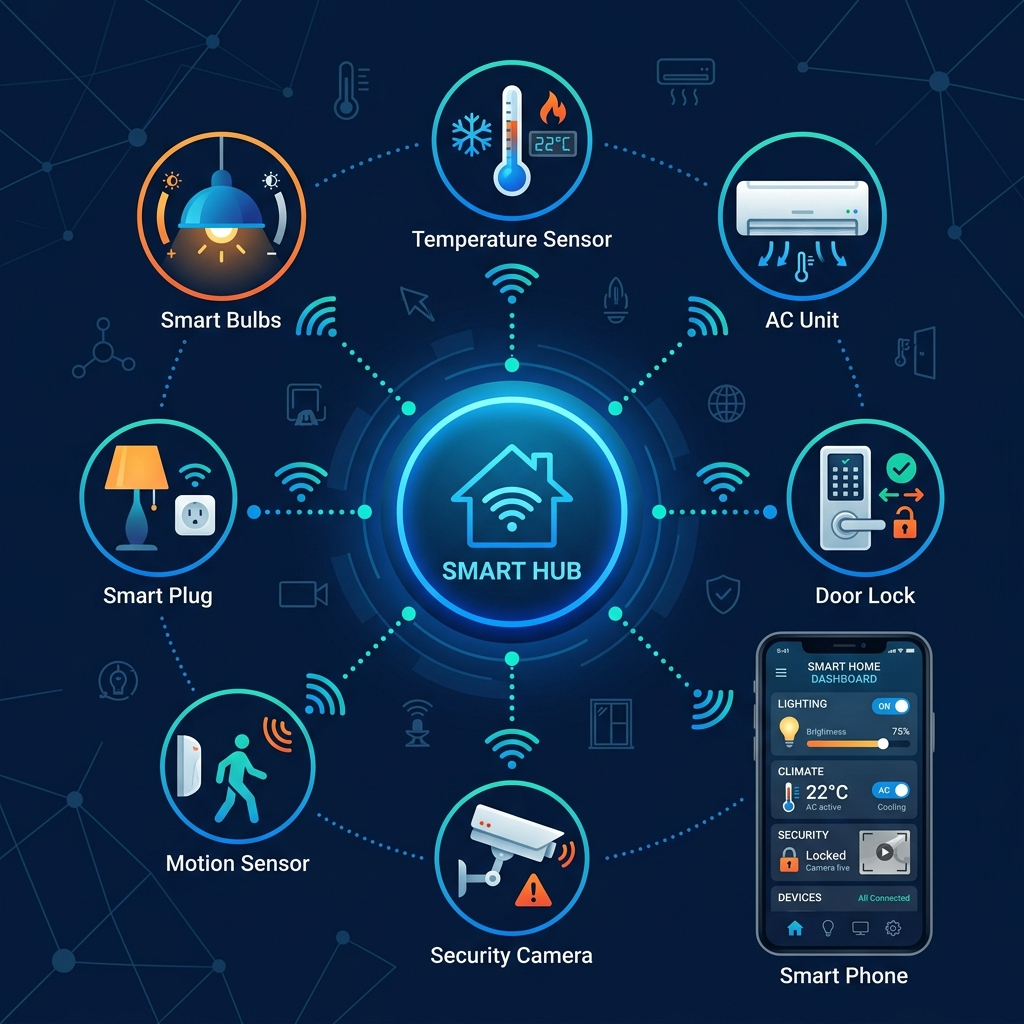
\includegraphics[width=0.5\textwidth]{images/architecture/smart_home_concept.png}
\caption{Smart Home Automation Concept}
\label{fig:smart_home_concept}
\end{figure}

\section{Problem Statement}

Traditional home automation systems face several critical limitations:

\begin{itemize}
    \item \textbf{Manual Operation:} Most households still rely on physical switches and manual controls, requiring occupants to be physically present to control devices.
    
    \item \textbf{No Remote Access:} Devices cannot be controlled from outside the home, leading to inconvenience and security concerns (e.g., inability to turn off forgotten appliances).
    
    \item \textbf{Lack of Automation:} Without automated routines, users must manually perform repetitive control sequences, consuming time and effort.
    
    \item \textbf{Energy Wastage:} Devices often remain active longer than necessary due to the absence of intelligent scheduling or environmental awareness, leading to increased energy consumption and costs.
    
    \item \textbf{Cloud Dependency:} Many existing solutions require constant cloud connectivity, making them unreliable during network outages or when cloud infrastructure is unavailable.
    
    \item \textbf{High Costs:} Commercial smart home systems often require expensive subscriptions and proprietary hardware, making them inaccessible to average users.
\end{itemize}

\section{Project Objectives}

This project aims to design and implement an affordable, user-friendly, and reliable smart home automation system with the following objectives:

\begin{enumerate}
    \item Develop a complete smart home control system comprising:
    \begin{itemize}
        \item An Android application for intuitive user interaction
        \item ESP32-based firmware for relay control and sensor integration
        \item Cloud infrastructure for real-time synchronization
    \end{itemize}
    
    \item Enable remote control of multiple relay-based devices through a mobile application
    
    \item Implement offline-first architecture with local caching to ensure functionality during network outages
    
    \item Support BLE-based device provisioning without requiring cloud connectivity during initial setup
    
    \item Provide environmental monitoring through temperature and humidity sensors
    
    \item Enable creation of automated routines based on environmental conditions and time-based schedules
    
    \item Implement per-device runtime tracking for energy consumption awareness
    
    \item Support multiple device instances (4, 6, and 8-channel relay variants) with unified firmware
\end{enumerate}

\section{Project Scope}

\subsection{What is Included}

\begin{itemize}
    \item Android mobile application with MVVM architecture and Compose UI
    \item ESP32 firmware supporting relay control, touch inputs, and sensor polling
    \item Firebase RTDB integration for cloud synchronization
    \item BLE-based device discovery and provisioning
    \item Automation engine for rule-based device control
    \item Schedule management system with conflict prevention
    \item Scene-based control for coordinated device actions
    \item User authentication via Google Sign-In
    \item Environment sensor integration (temperature and humidity)
\end{itemize}

\subsection{What is Excluded}

\begin{itemize}
    \item Voice assistant integration (future enhancement)
    \item Matter protocol support (future enhancement)
    \item AI-based automation suggestions (future enhancement)
    \item Advanced analytics and energy cost prediction (basic tracking only)
    \item Multi-user household role management (owner-only in V1)
    \item Home Assistant or third-party ecosystem bridges (future consideration)
\end{itemize}

\section{Motivation}

The motivation for this project stems from multiple factors:

\begin{enumerate}
    \item \textbf{Accessibility:} Most smart home solutions are expensive and vendor-locked. This project demonstrates that a feature-rich system can be built using affordable, open-source components (ESP32, open-source libraries, free Firebase tier).
    
    \item \textbf{Reliability:} By implementing offline-first caching and local command queueing, the system continues functioning during network outages—addressing a critical gap in cloud-dependent commercial solutions.
    
    \item \textbf{Privacy:} Users maintain control over their data with clear delineation between on-device processing and cloud synchronization, reducing privacy concerns compared to proprietary ecosystems.
    
    \item \textbf{Learning Opportunity:} This project integrates multiple technologies—embedded systems, mobile development, cloud infrastructure, and IoT—providing a comprehensive real-world engineering experience.
    
    \item \textbf{Practical Impact:} Smart home automation directly improves quality of life through convenience, security, and energy efficiency.
\end{enumerate}

\section{Report Organization}

This report is structured as follows:

\begin{itemize}
    \item \textbf{Chapter 2:} Literature Survey—comparison of existing smart home systems and identification of research gaps
    
    \item \textbf{Chapter 3:} System Architecture and Design—overall system architecture, provisioning flow, presence awareness, database design, and data flow
    
    \item \textbf{Chapter 4:} Hardware Design—component selection, circuit design, and GPIO configuration
    
    \item \textbf{Chapter 5:} Software Design and Implementation—Android architecture, application screens, firmware modules, and automation engine
    
    \item \textbf{Chapter 6:} Testing and Validation—test cases, test results, and validation methodology
    
    \item \textbf{Chapter 7:} Results and Discussion—performance metrics and analysis
    
    \item \textbf{Chapter 8:} Future Scope—planned enhancements and extensions
    
    \item \textbf{Chapter 9:} Conclusion—summary of achievements and lessons learned
\end{itemize}
